
% 微分方程的数值方法

\chapter{EM数值方法}

\section{假设}
\begin{assumption}\label{Lipschitz}
	在这一章节中, 我们假设SDE\cref{basic SDE}的漂移项系数$f$满足全局\textnormal{Lipschitz}条件的, 即存在一个常数$K>0$, 使得
	\begin{equation}
		|f(x)-f(y)| \le K|x-y|. 
	\end{equation}
\end{assumption}

\begin{assumption}\label{linear growth}
	在这一章节中, 我们假设SDE\cref{basic SDE}的漂移项系数$f$满足线性增长条件, 即存在一个常数$K>0$, 使得
	\begin{equation}
		|f(x)| \le K(1+|x|). 
	\end{equation}
\end{assumption}

%\begin{assumption}\label{moment}
%	令$T>0$,假设漂移项系数$f$是二阶连续可微的并且满足:
%	\begin{equation}
%		\sup\limits_{t\in[0,T]}\mathbb{E}\left|f'(x(t))\right|+
%		\sup\limits_{t\in[0,T]}\mathbb{E}\left|f'(x(t))f(x(t))+
%		\frac{\sigma^2}2f''(x(t))\right|<\infty.
%	\end{equation}
%\end{assumption}

\begin{assumption}\label{momentEM}
	在这一章节中, 我们假设SDE\cref{basic SDE}的漂移项系数$f$是二阶连续可微的, 并且存在常数$K>0$使得
	\begin{equation}
		|f(x)f'(x)| + |\sigma f'(x)| + |\sigma^2 f''(x)| \leq K(1 + |x|).
	\end{equation}
	
\end{assumption}

\section{等距步长的EM数值方法}


下面的命题致力于推导 \( \sup_{0 \leq r \leq T} |X_r| \) 的 \( p \) 阶矩存在的充分条件,其中 \( X \) 是 SDE\cref{basic SDE} 的解。这些条件对于本论文主要定理的建立是必要的。
\textcolor{red}{理论上这个可以扩展到所有的正数p吧。ifthen 下面的单边lip的的系数可以满足任何的次/超线性增长。当然如果我们能证明下面的那些实际上是满足超线性的话,那么就可以直接得到了,这里就不需要扩展了。}
\begin{proposition}\label{main pro1}
	令X是SDE\cref{basic SDE}的解, 其中f满足\cref{Lipschitz}和\cref{linear growth}, 那么对于任意的$p \ge 1$, 存在常数$c_1,c_1$, 使得$\mathbb{E}_{B}[Y_T^{(p)}] < c_1 e^{c_2E_T }. $, 其中$Y_t^{(p)} := 1 + \sup\limits_{0\le r\le t}|X_r|^p$, .
\end{proposition}
\begin{proof}
	设 $S_{\ell} := \inf\{ t \geq 0 : Y_{t}^{(p)} > \ell \}$,其中 $\ell \in \mathbb{N}$。由于解 $X$ 具有连续的路径,对每个 $t \geq 0$,$Y_{t}^{(p)} < \infty$,因此,随着 $\ell \to \infty$,$S_{\ell} \uparrow \infty$。对于 $\mathbb{P}_D$ 几乎处处的路径,我们首先将 Gronwall 型不等式应用于函数 $t \mapsto \mathbb{E}_B[Y_{t \wedge S_{\ell}}^{(p)}]$ 对于固定的 $\ell$,然后令 $t = T$ 并在得到的不等式中让 $\ell \to \infty$ 来建立 $\mathbb{E}_B[Y_T^{(p)}]$ 的上界。请注意,由于 $S_{\ell}$ 的定义,
	\[
	\int_{0}^{t} \mathbb{E}_B[Y_{r \wedge S_{\ell}}^{(p)}] \, dE_r \leq \ell E_t < \infty,
	\]
	这使得我们可以安全地应用 Gronwall 型不等式。
	
	假设 $p \geq 2$,因为对于 $1 \leq p < 2$ 的结果可以直接通过应用 $p \geq 2$ 时的结果和 Jensen 不等式得到。根据时间变换的Itô 公式,有 $X_s^p = x_0^p + J_s + K_s$,其中
	\[
	J_s := \int_0^s \sigma p X_r^{p-1}  \, dB_{E_r};
	\]
	\[
	K_s := \int_0^s \left\{ p X_r^{p-1} f(X_r) + \frac{\sigma^2}{2} p (p-1) X_r^{p-2}  \right\} \, dE_r.
	\]
	固定 $t \in [0, T]$ 和 $\ell \in \mathbb{N}$。根据\cref{linear growth} 以及不等式 $(x + y + z)^p \leq c_p (x^p + y^p + z^p)$,其中 $x, y, z \geq 0$ 且 $c_p = 3^{p-1}$,有
	\[
	\mathbb{E}_B\left[ \sup_{0 \leq s \leq t \wedge S_{\ell}} |K_s| \right] \leq \left( p c_p K + \frac{1}{2} p(p-1) c_p K^2 \right) \int_0^{t \wedge S_{\ell}} \mathbb{E}_B[Y_r^{(p)}] \, dE_r.
	\]
	由于 $(J_s)_{s \geq 0}$ 是一个局部鞅,应用 BDG 不等式得到
	\[
	\mathbb{E}_B\left[\sup_{0 \leq s \leq t \wedge S_{\ell}} |J_s| \right] \leq b_1 \mathbb{E}_B \left[\left( \int_0^{t \wedge S_{\ell}} \sigma^2 p^2 X_r^{2p-2}  \, dE_r \right)^{1/2}\right],
	\]
	因此,
	\[
	\mathbb{E}_B \left[\sup_{0 \leq s \leq t \wedge S_{\ell}} |J_s| \right] \leq b_1 \mathbb{E}_B \left[ p c_p K \left( Y_{t \wedge S_{\ell}}^{(p)} \int_0^{t \wedge S_{\ell}} Y_r^{(p)} \, dE_r \right)^{1/2} \right]
	\]
	\[
	\leq \frac{1}{2} \mathbb{E}_B \left[Y_{t \wedge S_{\ell}}^{(p)}\right] + 2b_1^2 p^2 c_p^2 K^2 \int_0^{t \wedge S_{\ell}} \mathbb{E}_B \left[Y_r^{(p)}\right] \, dE_r,
	\]
	其中最后一个不等式由基本不等式 $(ab)^{1/2} \leq a/\lambda + \lambda b$ 导出,适用于任意 $a, b, \lambda > 0$,且 $\lambda := 2b_1 p c_p K$. 
	注意,对于任意非负过程 $(L_t)_{t \geq 0}$,都有
	\[
	\int_0^{t \wedge S_{\ell}} L_r \, dE_r \leq \int_0^t L_{r \wedge S_{\ell}} \, dE_r.
	\]
	确实,当 $t \leq S_{\ell}$ 时,不等式显然成立,而如果 $t > S_{\ell}$,则
	\[
	\int_0^{S_{\ell}} L_r \, dE_r + \int_{S_{\ell}}^t L_{S_{\ell}} \, dE_r \geq \int_0^{t \wedge S_{\ell}} L_r \, dE_r.
	\]
	因此,通过上面对 $J_s$ 和 $K_s$ 的估计,有
	\[
	\mathbb{E}_B[Y_{t \wedge S_{\ell}}^{(p)}] \leq 2(1 + |x_0|^p) + 2K^2\left(p c_p K + \left(p(p-1) c_p / 2 + 2b_1^2 p^2 c_p^2\right) \right)\int_0^t \mathbb{E}_B[Y_{r \wedge S_{\ell}}^{(p)}] \, dE_r,
	\]
	通过应用Gronwall 型不等式,得到
	\[
	\mathbb{E}_B[Y_{t \wedge S_{\ell}}^{(p)}] \leq 2(1 + |x_0|^p) e^{2K^2E_T\left(p c_p K + \left(p(p-1) c_p / 2 + 2b_1^2 p^2 c_p^2\right) \right) }.
	\]
	令 $t = T$,并让 $\ell \to \infty$,由于 $\xi(u)$ 不依赖于 $\ell$,并应用单调收敛定理,可得
	
	\begin{equation}\label{boundY}
			\mathbb{E}_B[Y_T^{(p)}] \leq 2(1 + |x_0|^p) e^{2K^2E_T \left(p c_p K + \left(p(p-1) c_p / 2 + 2b_1^2 p^2 c_p^2\right) \right)}. 
	\end{equation}
%	对两边取期望$\mathbb{E}_D$, 得到 $\mathbb{E}[Y_T^{(p)}] \leq \mathbb{E}[ce^{cE_T}] < \infty$,这归因于 \cite{jin2019strong}中定理 1的结果。
	
\end{proof}

回顾一下,假设 \( X_t\) 是一个步长为 \( \delta > 0 \) 的逼近过程,如果存在有限的正常数,使得对于所有 足够小的\( \delta \) ,有$\mathbb{E} \left[\sup\limits_{0\le t \le T}|X(t) - X_t|\right] \leq C\delta^{\eta}$, 则我们称 \( X_t \) 强收敛于解 \( X(t) \) 并且收敛阶数为 \( \eta \).

对于随机微分方程\cref{basic SDE},它的EM数值格式是:
\begin{equation}\label{EMmethod}
	X_{t_{i+1}}=X_{t_i}+f(X_{t_{i}})\Delta E_{i}+\sigma\Delta B_{E_{i}},\quad i=0,1,2,\ldots,\qquad X_0=X(0)
\end{equation}
其中$\Delta E_{i}=E(t_{i+1})-E(t_i)$以及$\Delta B_{E_{i}}=B(E{(t_{i+1})})-B(E({t_i}))$.

\begin{theorem}\label{main th EM}
	对于任意的常数$\epsilon>0$, 令$\epsilon < T_1 < T_2, \lceil T_1/\Delta t \rceil = m$和$\lceil T_2/\Delta t \rceil = n$, 在 \textnormal{\cref{Lipschitz}}, \textnormal{\cref{linear growth}}和\textnormal{\cref{momentEM}}的条件下, 存在常数C, 使得下面的不等式成立:
	$$\mathbb{E}\left[\sup\limits_{i = m,m+1,\ldots ,n} |X({t_i})-X_{t_i}|\right]\le C\Delta t^\alpha$$
\end{theorem}
\begin{proof}
	
	考虑SDE \eqref{basic SDE}在$[t_i, t_{i+1})$的积分:
	\begin{align}
		\int_{t_i}^{t_{i+1}}dX(s)=\int_{t_i}^{t_{i+1}}f(X(s))dE(s)+\int_{t_i}^{t_{i+1}}\sigma dB(E(s)). 
	\end{align}
	由时间变换的变量变换公式\cite{kobayashi2011stochastic}, 上式等价于
	\begin{align}\label{eq:4}
		\int_{t_i}^{t_{i+1}}dX(s))=\int_{E_{t_i}}^{E_{t_{i+1}}}f(X(D(s-)))ds+\int_{t_i}^{t_{i+1}}\sigma dB(E(s)). 
	\end{align}
	针对于漂移项$f(X(D(s-)))$, 下面等式恒成立:
	\begin{align}\label{eq:ito}
		\int_{E(t_i)}^{E(t_{i+1})} f(X(D(t-)))) - f(X(D(t_i-))) dt = \int_{E(t_i)}^{E(t_{i+1})} \int^{D(t-)}_{D(t_i-)} df(X(s)) dt. 
	\end{align}
	由\cref{ito}的时间变换It\^{o}公式, 于是\eqref{eq:ito}变成
	\begin{equation}\label{eq:ito1}
		\begin{aligned}
			&\quad\int_{E(t_i)}^{E(t_{i+1})} f(X(D(t-))) - f(X(D(t_i-))) dt \\
			&= \int_{E(t_i)}^{E(t_{i+1})} \int_{t_i}^{t} \left( f(X(D(s-))) f^{\prime}(X(D(s-))) + \frac{1}{2} \sigma^2 f^{\prime\prime}(X(D(s-))) \right) ds \, dt\\
			&\quad + \int_{E(t_i)}^{E(t_{i+1})} \int_{t_i}^{t} \sigma f^{\prime}(X(D(s-))) \, dB(s) \, dt . 
		\end{aligned}
	\end{equation}
	由\eqref{eq:4}与\eqref{eq:ito1}, 以及时间变换的变量变换公式可以得到
	\begin{align*}
		X(t_{i+1}) 
		&= X(t_i) + \int_{E(t_i)}^{E(t_{i+1})} f(X({D(t_i-)})) \, dt + \int_{t_i}^{t_{i+1}} \sigma \, dB(E(t)) \\
		&\quad + \int_{E(t_i)}^{E(t_{i+1})} \int_{t_i}^{t}\left( f(X(D(s-))) f^{\prime}(X(D(s-))) + \frac{1}{2} \sigma^2 f^{\prime\prime}(X(D(s-))) \right) ds \, dt \\
		&\quad + \int_{E(t_i)}^{E(t_{i+1})} \int_{t_i}^{t}\sigma f^{\prime}(X(D(s-)))) \, dB(s) \, dt \\
		&= X(t_i) + \int_{t_i}^{t_{i+1}} f(X({t_i)}) \, dE(t) + \int_{t_i}^{t_{i+1}} \sigma \, dB(E(t)) \\
		&\quad + \int_{t_i}^{t_{i+1}} \int_{E(t_i)}^{E(t)} \left( f(X(D(s-))) f^{\prime}(X(D(s-))) + \frac{1}{2} \sigma^2 f^{\prime\prime}(X(D(s-))) \right) ds \, dE(t) \\
		&\quad + \int_{t_i}^{t_{i+1}} \int_{E(t_i)}^{E(t)}\sigma f^{\prime}(X(D(s-))) \, dB(s) \, dE(t)\\
		&= X(t_i) + \int_{t_i}^{t_{i+1}} f(X({t_i})) \, dE(t) + \int_{t_i}^{t_{i+1}} \sigma \, dB(E(t)) \\
		&\quad + \int_{t_i}^{t_{i+1}} \int_{t_i}^{t} \left( f(X(s)) f^{\prime}(X(s)) + \frac{1}{2} \sigma^2 f^{\prime\prime}(X(s)) \right) dE(s) \, dE(t) \\
		&\quad + \int_{t_i}^{t_{i+1}} \int_{t_i}^{t}\sigma f^{\prime}(X(s)) \, dB(E(s)) \, dE(t). 
	\end{align*}
	因此
	\begin{align}\label{eq:3}
		X(t_{i+1})
		&= X(t_i) + \int_{t_i}^{t_{i+1}} f(X({t_i)}) \, dE(t) + \int_{t_i}^{t_{i+1}} \sigma \, dB(E(t)) + R_i. 
	\end{align}
	将$R_i$分解成$R_i = R_i^{(1)} + R_i^{(2)}$, 其中:
	\begin{align*}
		& R_i^{(1)} = \int_{t_i}^{t_{i+1}} \int_{t_i}^{t} \left( f(X(s)) f^{\prime}(X(s)) + \frac{1}{2} \sigma^2 f^{\prime\prime}(X(s)) \right) dE(s) \, dE(t), \\
		& R_i^{(2)} = \int_{t_i}^{t_{i+1}} \int_{t_i}^{t} \sigma f^{\prime}(X(s)) \, dB(E(s)) \, dE(t). 
	\end{align*}
	使用(\ref{eq:4})和\eqref{eq:3}可以得到:
	\begin{equation}
		X({t_{i+1}})-X_{t_{i+1}}=X({t_i})-X_{t_i}+(f{(x({t_i}))}-f{(x^\delta_{t_i})})\Delta E_{i}+R_{i}. 
	\end{equation}
	令$e_i = X({t_i})-X_{t_i}$, 由\cref{Lipschitz}得到:
	\begin{equation}
		|e_{s+1}|\leq(1+K{\Delta}E_{s})|e_{s}|+R_{s}, ~~\text{其中}s=m,\cdots ,n.
	\end{equation}
	由\cref{gronwall}, 可以得到$|e_n| \leq \sum\limits_{j=m-1}^{n-1}|R_{j+1}|\prod\limits_{l=j+1}^{n-1}|1+K\Delta E_l|$. 
	
	为了估计这个不等式,我们使用了逆从属过程 \( E(t) \) 路径几乎处处 Hölder 连续的事实。具体地,对于每个 \( 0 < \beta < 1 \),存在一个常数 \( C > 0 \),使得对于所有 \( t, s \)(当 \( t \neq s \) 时),有
	\begin{equation}\label{Einc}
		|E(t) - E(s)| \leq C |t - s|^\beta \quad \text{a.s.}
	\end{equation}

	其中,\( \beta \) 与 Lévy 过程 \( D(t) \) 的稳定指数 \( \alpha \) 相关,通常有 \( \beta \leq \alpha \)。这一 Hölder 连续性表明,逆过程 \( E(t) \) 的增量按照指数 \( \alpha \) 的速率衰减,因此 \( E(t) \) 展现出平滑的连续路径。于是, 
	\begin{equation*}
		\sup\limits_{k=m ,\ldots ,n} \prod\limits_{l=1}^{k}(1+K\Delta E_l) \leq \sup\limits_{k=m,\ldots, n} \prod\limits_{l=1}^{k}(1+C\Delta t^{\beta})
	\end{equation*}
	通过对$\Delta t$取极限, 
	于是
	\begin{equation*}
		\sup\limits_{k=m, \ldots, n. } \prod\limits_{l=1}^{k}(1+K\Delta E_l) < \infty
	\end{equation*}
	于是:
	\begin{equation}
		\mathbb{E}\left[\sup\limits_{k=m, \ldots, n}\left|e_k\right|\right] \leq C\mathbb{E}\sum_{j=0}^{n-1}|R_{j+1}| \leq C\mathbb{E}\sum\limits_{j=0}^{n-1}|R_{j+1}^{(1)}| + C\mathbb{E}\sum\limits_{j=0}^{n-1}|R_{j+1}^{(2)}|. 
	\end{equation}
	
	于是对于第一项,  由\cref{momentEM}, \cref{main pro1}和\cref{main lemma}, 可以得到
	\begin{align*}
		\mathbb{E} \left[|R_{j+1}^{(1)}| \right] &= \mathbb{E}_D \left[
		\int_{t_i}^{t_{i+1}} \int_{t_i}^{t}  \mathbb{E}_B \left( f(X(s)) f^{\prime}(X(s)) + \frac{1}{2} \sigma^2 f^{\prime\prime}(X(s)) \right) dE(s) \, dE(t)
		\right] \\
		&\le C\mathbb{E}_D \left[
		\int_{t_i}^{t_{i+1}} \int_{t_i}^{t}  \mathbb{E}_B \left[1+|X(s)| \right] dE(s) \, dE(t)
		\right] \\
		& \le C\mathbb{E}_D \left[
		\int_{t_i}^{t_{i+1}} \int_{t_i}^{t}  e^{E(T)} dE(s) \, dE(t)
		\right] 
	\end{align*}
	这里的最后一个不等式是由于\cref{boundY}.由于$E_t$是$\mathcal{G}_t$可测的, 并且满足\cref{slowerthant}, 于是存在$T>0$使得$E_T < T $. 同样的当$t \le T$, 我们可以得到
	\begin{equation}\label{boundE}
		E_t \leq E_T \leq T,
	\end{equation}
	因此我们可以得到
	\begin{equation*}
		\mathbb{E} \left[|R_{j+1}^{(1)}| \right]  \le C\mathbb{E}_D \left[
		\int_{t_i}^{t_{i+1}} \int_{t_i}^{t}  e^T dE(s) \, dE(t)
		\right] \le C\Delta t^{1+\alpha}. 
	\end{equation*}
	 于是, 我们利用期望的线性性质, 可以得到
	\begin{equation}\label{R1}
		\mathbb{E}\sum\limits_{j=0}^{n-1}|R_{j+1}^{(1)}|= \sum\limits_{j=0}^{n-1}\mathbb{E}|R_{j+1}^{(1)}| \leq
		C\sum\limits_{j=0}^{n-1}\Delta t^{1+\alpha} \le C\Delta t^\alpha. 
	\end{equation}
	
	对于第二项$\mathbb{E}|\sum\limits_{j=0}^{n-1}R_{j+1}^{(2)}|$, 
	通过BDG不等式和\cref{main lemma}可以得到
%	\begin{equation}\label{dEdB}
%		\mathbb{E}[dB_EdE]^2=\mathbb{E}[(dB_E)^2(dE)^2]=\mathbb{E}_D[(dE)^2\mathbb{E}_B(dB_E)^2]\leq
%		C\mathbb{E}_{D}[dE]^3\leq C\Delta t ^{1+2\alpha}. 
%	\end{equation}
	于是, 
	\begin{align*}
		\mathbb{E} \left[|R_{j+1}^{(2)}| \right] &= \mathbb{E}_D \left[
		\int_{t_i}^{t_{i+1}} \mathbb{E}_B  \left[\int_{t_i}^{t}  \sigma f^{\prime}(X(s)) dB_{E(s)}\right] \, dE(t)
		\right] \\
		& \le C\mathbb{E}_D \left[
		\int_{t_i}^{t_{i+1}} \left[\int_{t_i}^{t}  \mathbb{E}_B\left(\sigma f^{\prime}(X(s))\right)^2 dE(s)\right]^{\frac{1}{2}} \, dE(t)
		\right] \\
		& \le C\mathbb{E}_D \left[
		\int_{t_i}^{t_{i+1}} \left[\int_{t_i}^{t}  	\mathbb{E}_B \left[1+|X(s)|\right]^2 dE(s)\right]^{\frac{1}{2}} \, dE(t)
		\right] \\
		&\le C \mathbb{E}_D \left[
		\int_{t_i}^{t_{i+1}} \left[\int_{t_i}^{t}  e^{2E(T)} dE(s)\right]^{\frac{1}{2}} \, dE(t)\right]\\
		&\le C \left\{\mathbb{E}_D \left[
		\int_{t_i}^{t_{i+1}} \left[\int_{t_i}^{t}  e^{2E(T)} dE(s)\right]^{\frac{1}{2}} \, dE(t)\right]^2\right\}^{\frac{1}{2}}\\
		&\le C\Delta t^{\frac{1}{2}+\alpha}. 
	\end{align*}
	使用Cauchy-Schwarz不等式,可以得到:
	\begin{equation}\label{R2}
		\mathbb{E}\left|\sum_{j=0}^{n-1}R_{j+1}^{(2)}\right|  \le C\mathbb{E} \left|\sum_{j=0}^{n-1}(R_{j+1}^{(2)})^2\right|^{\frac{1}{2}} \le C\sqrt{\sum_{j=0}^{n-1}\mathbb{E}(R_{j+1}^{(2)})^2}
		\le C\sqrt{\sum_{j=0}^{n-1}\Delta t^{1+2\alpha}} \le C\Delta t^{\alpha}. 
	\end{equation}
	
	于是结合\cref{R1}和\cref{R2}, 得到
	$$\mathbb{E}\left[\sup\limits_{k=m \ldots n}\left|e_k\right|\right] \leq C\Delta t^\alpha. $$
\end{proof}


	
\section{随机步长的EM数值方法}

%设定等距步长 $\delta \in (0,1)$ 及时间区间 $T > 0$.为了在区间 $[0,T]$ 上逼近逆从属过程 $E$,我们遵循 \cite{magdziarz2009stochastic} 中提出的方法.具体来说,首先通过模拟具有独立且平稳增量的从属过程 $D$ 的样本路径来进行逼近.设定 $D_0 = 0$,然后遵循规则 $D_{i\delta} := D_{(i-1)\delta} + Z_i, i=1,2,3,\ldots$,其中 $\{Z_i\}_{i \in \mathbb{N}}$ 为独立同分布的序列,且 $Z_i \stackrel{d}{=} D_{\delta}$.我们在找到整数 $N$ 使得 $T \in [D_N\delta, D_{(N+1)\delta})$ 时停止该过程.请注意,$\mathbb{N}\cup\{0\}$ 值的随机变量 $N$ 确实存在,因为 $D_t \to \infty$ 随着 $t \to \infty$ 几乎必然成立.可以通过下面的算法生成随机变量 $\{Z_i\}$,
%\begin{align*}
%	Z(i)=\delta^{1/\alpha}\xi_{i}
%\end{align*}
%其中$\xi_i$是独立同分布的完全偏斜的$\alpha$稳定随机变量,$\xi_i$的实现过程如下:
%\begin{align*}
%	\xi_i=\frac{\sin(\alpha(V+c_1))}{\left(\cos(V)\right)^{1/\alpha}}\Big(\frac{\cos(V-\alpha(V+c_1))}{W}\Big)^{(1-\alpha)/\alpha}
%\end{align*}
%其中$c_1 = \frac{\pi}{2}$,随机变量$V$是$(-\frac{\pi}{2},\frac{\pi}{2})$上的均匀分布,$W$是均值为$1$的指数分布.
%然后,令
%$$
%E_t^\delta := \left(\min\{n \in \mathbb{N}; D_{n\delta} > t\} - 1\right)\delta, \quad t \in [0, T].
%$$
%过程 $E^\delta = (E_t^\delta)_{t \geq 0}$ 的样本路径是具有恒定跳跃大小 $\delta$ 的单调递增阶梯函数,第 $i$ 个等待时间为 $Z_i = D_{i\delta} - D_{(i-1)\delta}$.过程 $E^\delta$ 有效地逼近 $E$;实际上,几乎必然地,
%\begin{equation}
%	E_t - \delta \leq E_t^\delta \leq E_t \quad \text{对于所有} \quad t \in [0, T].
%\end{equation}


首先,我们描述一种用于逆从属过程 \( E \) 的近似方法,该方法在 [15,16] 中给出。固定等距步长 \(\delta > 0\) 和时间区间 \( T > 0 \)。为了在区间 \([0, T]\) 上近似 \( E \),我们首先模拟从属过程 \( D \) 的样本路径,该过程具有独立且平稳的增量,设定 \( D_0 = 0 \),然后按照规则 \( D_i^\delta := D_{i-1}^\delta + Z_i \),其中 \( i = 1, 2, 3, \ldots \),并且 \( (Z_i)_{i \in \mathbb{N}} \) 是一个 i.i.d. 序列,且每个 \( Z_i \) 都服从分布 \( Z = \Delta D_\delta \)。我们在找到满足 \( T \in [D_{N\delta}, D_{(N+1)\delta}) \) 的整数 \( N \) 时停止这个过程。请注意,\( \mathbb{N} \)-值的随机变量 \( N \) 确实存在,因为几乎必然 \( D_t \to \infty \) 当 \( t \to \infty \) 时。为了生成随机变量 \( (Z_i) \),可以使用 [2] 第六章中给出的算法。接下来,定义 \( E^\delta := (\min(n \in \mathbb{N}; D_{n\delta} > t) - 1) \delta \)。过程 \( E^\delta = (E_t^\delta)_{t \geq 0} \) 是非递减的阶梯函数,具有常数跳跃大小 \(\delta\),并且第 \( i \)-次等待时间为 \( Z_i = D_i^\delta - D_{i-1}^\delta \)。事实上,很容易看出,对于 \( n = 0, 1, 2, \ldots, N \),当 \( t \in [D_{n\delta}, D_{(n+1)\delta}) \) 时,\( E^\delta = n\delta \)。特别地,\( E^\delta = N\delta \)。如 [10,16] 所述,过程 \( E^\delta \) 有效地近似 \( E \);即,几乎必然地,
\[
E_t - \delta \leq E^\delta \leq E_t \quad \text{对于所有} \quad t \in [0, T].
\]
现在,对于 \( n = 0, 1, 2, \ldots, N \),设定
\[
\tau_n = D_{n\delta}.
\]

根据 \( B \) 和 \( D \) 之间的独立假设,我们可以在时间步长 \(\{0, \delta, 2\delta, \ldots, N\delta\}\) 上近似布朗运动 \( B \)。基于这一点,定义离散时间过程 \(\left(X_{\tau_n}\right)_{n\in\{0,1,2,\ldots, N\}}\) 为 \( X_0 := x_0 \),对于 \( n = 0, 1, 2, \ldots, N-1 \),有

\begin{equation}\label{stostep}
	X_{\tau_{n+1}} := X_{\tau_n}  + f\left(X_{\tau_n}\right)\left(E_{\tau_{n+1}}-E_{\tau_n}\right)  + \sigma\left(B_{E_{\tau_{n+1}}}-B_{E_{\tau_n}}\right).
\end{equation}


由于关系 \( E_{\tau_{n}} = n\delta \),上述等式等价于
\begin{equation}\label{nostostep}
	X_{\tau_{n+1}} :=X_{\tau_n}  + f\left(X_{\tau_n}\right)\delta + \sigma\left(B_{(n+1)\delta}-B_{n\delta}\right).
\end{equation}

注意,尽管表达式\cref{nostostep}看起来像是采取了非随机时间步长,但实际上我们确实采取了随机时间步长 \(\tau_0, \tau_1, \tau_2, \ldots, \tau_N\) 来离散化驱动过程 \( E = \left(E_t\right)_{t \geq 0} \) 和 \( B \circ E = \left(B_{E_t}\right)_{t \geq 0} \),如\cref{stostep}中所示;因此,时间变化过程的随机捕捉事件的关键特性(即产生常数时间段的部分)实际上是由随机步长 \(\tau_{n+1} - \tau_n = D_{(n+1)\delta} - D_{n\delta} = \Delta D_{\delta}\) 所捕捉的。\textbf{\{}此外,注意我们并没有通过非随机时间步长来离散化 SDE;如果这样做会变得非常困难,因为驱动过程 \( E \) 和 \( B \circ E \) 都没有独立增量,也没有平稳增量。\textbf{\}}

为了定义一个连续时间过程 \(\left(X_t\right)_{t\in[0, T]}\),我们采用连续插值;即,当 \(s \in \left[\tau_n, \tau_{n+1}\right)\) 时,

\begin{equation}
	X_s:= X_{\tau_n} +  \int_{\tau_n}^s f\left(X_{\tau_n}\right) \, dE_r + \int_{\tau_n}^s \sigma dB_{E_r}.
\end{equation}


定义

\[
n_t = \max\left\{n \in \mathbb{N} \cup \{0\}; \tau_n \leq t\right\} \text{ 对于 } t \geq 0.
\]

那么显然对于任何 \( t > 0 \),都有 \( \tau_{n_t} \leq t < \tau_{n_t+1} \)。利用\cref{nostostep}和恒等式 \( X_s - x_0 = \sum_{i=0}^{n_s-1} \left(X_{\tau_{i+1}} - X_{\tau_i}\right) + \left(X_s - X_{\tau_{n_s}}\right) \),我们可以将 \( X_s - x_0 \) 表示为

\[
\sum_{i=0}^{n_s-1} \left[ f\left(E_{\tau_i}, X_{\tau_i}\right)\delta + \sigma\left(B_{(i+1)\delta} - B_{i\delta}\right)\right] + \left(X_s - X_{\tau_{n_s}}\right).
\]

其中我们使用了 \( i\delta = E_{D_{i\delta}} = E_{\tau_i} \)。利用\cref{intX}以及事实 \(\tau_i = \tau_{n_r}\) 对于任意 \( r \in [\tau_i, \tau_{i+1}) \),我们可以将后者重新写成如下便于处理的形式:
\begin{equation}\label{intX}
	X_s = x_0 + \int_{0}^{s} f\left(X_{\tau_{n_r}}\right) \, dE_r + \int_{0}^{s} \sigma \, dB_{E_r}.
\end{equation}

%在\cite{jin2019strong}中对$\Delta E$的处理时,t每次跳$D_{n\delta} - D_{(n-1)\delta}$,于是$E$每次对应改变$\delta$.然而,在我们的离散格式中,选择对t做等距离散,让t每次跳跃的长度是固定的长度h,于是$E$在第i次跳跃对应的变化就是$E_{ih} - E_{(i-1)h}$,这样的离散会导致出现$\Delta E=0$,这是得到收敛阶是$\alpha$的关键.

接下来, 我们来证明本章节第二个重要定理. 
\begin{theorem}\label{main th EM1}
	设 $X$ 为SDE\textnormal{\cref{basic SDE} }的解,在 \textnormal{\cref{Lipschitz}}, \textnormal{\cref{linear growth}}和\textnormal{\cref{momentEM}}的条件下, 
	设 $X_t$ 为在 \textnormal{\cref{nostostep}}和\textnormal{\cref{intX}}中定义的 EM数值方法。则存在与 $\delta$ 无关的常数 $C > 0$,使得对所有 $\delta \in (0,1)$,
	\[
	\mathbb{E} \left[ \sup_{0 \leq s \leq T} | X(s) - X_s | \right] \leq C \delta。
	\]
	因此,$X_t$ 在 $[0, T]$ 上以 1 阶一致强收敛于 $X(t)$。
\end{theorem}

\begin{proof}
	类似于\cref{main th EM}, 通过 Itô 公式展开,可以得到
	\begin{align}\label{afterito}
		X(\tau_{n+1}) = X(\tau_n) +  \int_{\tau_n}^{\tau_{n+1}} f(X(\tau_n)) \, \mathrm{d}E_u + \int_{\tau_n}^{\tau_{n+1}} \sigma \, \mathrm{d}B_{E_u} + R_{(\tau_n, \tau_{n+1})}; 
	\end{align}
	\begin{align*}
		R_{(a,b)} :=&  \int_a^b \int_a^{v} \left( f(X(\tau_{n_{u}}))f'(X(\tau_{n_{u}})) + \frac{\sigma ^2}{2} f''(X(\tau_{n_{u}}))  \right) \, \mathrm{d}E_{u} \, \mathrm{d}E_{v} \\
		&+ \int_a^b \int_a^{v} \sigma f'(X(\tau_{n_{u}}))   \, \mathrm{d}B_{E_{u}} \,\nonumber \mathrm{d}E_{v},
	\end{align*}
	将\cref{intX}与\cref{afterito}相减, 可以得到
	$Z_t := \sup_{0 \leq s \leq t} | X(s) - X_s | \leq I_1 + I_2 $,其中
	
	$$
	\begin{aligned}
		&I_1 := \sup_{0 \leq s \leq t} \left| \int_0^s f(X(\tau_{n_u})) - f(X_{\tau_{n_u}})  \, \mathrm{d}E_u \right|; \\
		&I_2 := \sup_{0 \leq s \leq t} \left| \sum_{i=0}^{n_s - 1} R_{(\tau_{t}, \tau_{t+1})} + R_{(\tau_{n_s}, s)} \right|.
	\end{aligned}
	$$
	
	对于$I_1$, 可以由\cref{Lipschitz}得到
	\begin{equation}\label{I1}
		\mathbb{E}_B[I_1] \leq K \int_0^t \mathbb{E}_B[Z_u] \, \mathrm{d}E_u.
	\end{equation}

	主要的技术部分涉及余项 $I_2$,其中包含两个不同的双重积分:$\mathrm{d}E_{u} \, \mathrm{d}E_{v}$ 和 $\mathrm{d}B_{E_{u}} \, \mathrm{d}E_{v}$。我们将在下面逐一处理这些积分。
	
	对于第一个积分$ \mathrm{d}E_{u} \, \mathrm{d}E_{v}$,
	\begin{align}
		& \quad \mathbb{E}_B \left[\sup_{0 \leq s \leq t} \left| \int_0^s \int_{\tau_{n_v}}^{v} f(X(\tau_{n_{u}}))f'(X(\tau_{n_{u}}))  + \frac{\sigma^2}{2} f''(X(\tau_{n_{u}})) \, \mathrm{d}E_{u} \, \mathrm{d}E_{v} \right|\right] \nonumber \\
		&\leq  \frac{3}{2}K \mathbb{E}_B[Y_T^{(1)}] \int_0^t \int_{\tau_{n_{v}}}^{v} \, \mathrm{d}E_{u} \, \mathrm{d}E_{v} \nonumber \\
		&\leq  \frac{3}{2}K E_T \mathbb{E}_B[Y_T^{(1)}] \delta.  \label{I21}
	\end{align}
	这里出现$\delta$而不是$\delta^{\alpha}$的主要原因是我们采用的是随机离散的数值格式.
	
	另一方面,我们需要估计 $\mathbb{E}_B \left[\sup_{0 \leq s \leq t} |M_{n_s} + U_s|\right]$,其中 $M_0 := 0$,对于 $n \geq 1$,$M_n := \sum_{i=0}^{n-1} L_i$,
	$$
	L_i := \int_{\tau_i}^{\tau_{i+1}} \int_{\tau_i}^{v} \sigma f'(X(\tau_{n_{u}})) \, \mathrm{d}B_{E_{u}} \, \mathrm{d}E_{v}, \quad U_s := \int_{\tau_{n_s}}^s \int_{\tau_{n_s}}^{v} \sigma f'(X(\tau_{n_{u}})) \, \mathrm{d}B_{E_{u}} \, \mathrm{d}E_{v}.
	$$
	
	我们首先验证随机积分 $L_i, i=0,1,\ldots,n_t-1$ 关于 $\mathbb{P}_B$ 是不相关的。令 $i < j$,因此 $\tau_{i+1} \leq \tau_j$。观察到 $\mathbb{E}_B [L_i L_j] = \mathbb{E}_B \left[L_i \mathbb{E}_B [L_j | \mathcal{F}_{E_{\tau_j}}]\right]$。根据假设和估计 (3.4),
	
	$$
	\mathbb{E}_B \left[\int_{\tau_j}^{\tau_{j+1}} \left|\int_{\tau_j}^{v} \sigma f'(X(u))\, \mathrm{d}B_{E_{u}}\right|^2 \mathrm{d}E_{v}\right] \leq \delta^2 K^2 \mathbb{E}_B [Y_t^{(2)}] < \infty.
	$$
	
	因此,$\mathbb{E}_B \left[L_j | \mathcal{F}_{E_{\tau_j}}\right] = \int_{\tau_j}^{\tau_{j+1}} \mathbb{E}_B \left[\int_{\tau_j}^{v} \sigma f'(X(u))  \, \mathrm{d}B_{E_{u}} | \mathcal{F}_{E_{\tau_j}}\right] \mathrm{d}E_{v} = 0$,这是由于条件 Fubini 定理(参考文献 [26] 中的定理 27.17)和鞅性质,从而得到不相关性。另一方面,由于 $E$ 具有连续路径,变量变换公式(参考文献 [13] 中的定理 3.1)表明 $M_n$ 可以表示为
	
	$$
	\sum_{i=0}^{n-1} \int_{i\delta}^{(i+1)\delta} \int_{i\delta}^{E_{v}} \sigma f'(X(D_{u-})) \, \mathrm{d}B_{u} \, \mathrm{d}v。
	$$
	
	该表示式,以及参考文献 [12] 中引理 5.7.1 和 10.8.1 的证明,表明离散时间过程 $(M_n)_{n \geq 0}$ 是一个平方可积的 $((\mathcal{F}_{n\delta})_{n \geq 0}, \mathbb{P}_B)$-鞅,初始值为 0。因此,由 BDG 不等式 (3.2) 和 $L_i$ 的不相关性,
	
	$$
	\mathbb{E}_B \left[\sup_{0 \leq s \leq t} M_{n_s}^2\right] \leq b_2 \sum_{i=0}^{n_t-1} \mathbb{E}_B [L_i^2]。
	$$
	因此,由 Cauchy-Schwartz 不等式,
	\begin{align}
		\mathbb{E}_B\left[\sup_{0\leq s\leq t}M_{n_s}^2\right] 
		&\leq b_2\delta\sum_{i=0}^{n_t-1}\int_{\tau_i}^{\tau_{i+1}}\mathbb{E}_B
		\left[\int_{\tau_i}^{v}\left|\sigma f'(X(u))\right|^2\mathrm{d}E_{u}\right]
		\mathrm{d}E_{v} \nonumber \\
		&\leq2b_2\delta K^2\mathbb{E}_B[Y_T^{(2)}]\sum_{i=0}^{n_t-1}\int_{\tau_i}^
		{\tau_{i+1}}(E_{v}-E_{\tau_i})\mathrm{d}E_{v} \nonumber \\
		&\leq 2b_2E_TK^2\mathbb{E}_B[Y_T^{(2)}]\delta^2. \label{I221}
	\end{align}
	另一方面, 
	\begin{align}
	\mathbb{E}_B\left[\sup_{0\leq s\leq t}U_s^2\right]  
	&\leq\mathbb{E}_B\biggl[\sup_{0\leq s\leq t}(E_s-E_{\tau_{n_s}})\int_{\tau_{n_s}}^s\left|\int_{\tau_{n_s}}^{v}\sigma f'(X(u))\mathrm{d}B_{E_{u}}\right|^2\mathrm{d}E_{v}\biggr] \nonumber \\ &\leq\delta\int_0^t\mathbb{E}_B\left[\sup_{s\in[v,t]}\left|\int_{\tau_{n_s}}^{v}\sigma f'(X(u))\mathrm{d}B_{E_{u}}\right|^2\right]\mathrm{d}E_{v}.\label{I222}
	\end{align}
	由于$\{(\tau_{n_s},v)~:~v~\leq~s~\leq~t\}~\subset~\{(\tau_{n_{v}},r)~:~\tau_{n_{v}}~\leq~r~\leq~s\},$于是
	\begin{align*}
	&\quad\mathbb{E}_B\Big[\sup_{s\in[v,t]}\Big|\int_{\tau_{n_{s}}}^{v}\sigma f'(X(u))\mathrm{d}B_{E_{u}}\Big|^2\Big]  \\
	&\le \mathbb{E}_B\left[\sup_{r\in[\tau_{n_{v}},v]}\left|\int_{\tau_{n_{v}}}^r\sigma f'(X(u))\mathrm{d}B_{E_{u}}\right|^2\right] \\
	&\leq b_2\mathbb{E}_B\left[\int_{\tau_{n_{v}}}^{r}\left|\sigma f'(X(u))\right|^2\mathrm{d}E_{u}\right]\\
	&\leq 2b_2K^2\mathbb{E}_B[Y_T^{(2)}]\delta.
	\end{align*}
	因此,\cref{I222}的上界为  $2b_2E_TK^2\mathbb{E}_B[Y_T^{(2)}]\delta^2.$ 将其与 \cref{I221} 结合得:
	\begin{equation}\label{I22}
					\mathbb{E}_B\left[\sup_{0\leq s\leq t}|M_{n_s}+U_s|^2\right] 
		\leq 8b_2E_TK^2\mathbb{E}_B[Y_T^{(2)}]\delta^2. 
	\end{equation}
	根据估计 \cref{I21} 和 \cref{I22},
	\begin{equation}\label{I2}
		\mathbb{E}_B[I_2] 
		\leq \left\{\frac{3}{2}E_T\mathbb{E}_B[Y_T^{(1)}]+(8b_2E_T\mathbb{E}_B[Y_T^{(2)}])^{1/2}\right\}K\delta. 
	\end{equation}
	
	现在,将 \cref{I1}和 \cref{I2}与  $\mathbb{E}_B[Y_T^{(1)}]\leq\sqrt{2}\mathbb{E}_B[Y_T^{(2)}]^{1/2}$ 结合得:
	\begin{equation*}
			\mathbb{E}_B[Z_t] 
		\leq \xi_2(E_T)\mathbb{E}_B[Y_T^{(2)}]^{1/2}\delta + K\int_0^t\mathbb{E}_B[Z_u] \mathrm{d}E_u.
	\end{equation*}

	其中 $\xi_2(u) := K(\frac{3\sqrt{2}}{2}u + (8b_2u)^{1/2}).$
	应用 Gronwall 类型不等式, 对两边取 $ \mathbb{E}_D $并使用 Cauchy-Schwartz 不等式得 
	\begin{equation*}
			\mathbb{E}[Z_T] \leq \mathbb{E}[\xi_2^4(E_T)]^{1/4}\mathbb{E}[(Y_T^{(2)})^2]^{1/4}\mathbb{E}[e^{2KE_T}]^{1/2}\delta.
	\end{equation*}
	由于对于任意的$\lambda>0, t>0,n>0$, 都有$\mathbb{E}[e^{\lambda E_t}] < \infty$, 以及$\mathbb{E}[E^n(t)] < \infty$, 再结合\cref{main pro1}, 于是可以得到该定理成立.
\end{proof}

	\begin{remark}
		从定理的结论可以看出来, 对于同样的EM数值方法, 由于步长选取方式的不同, 得到的收敛阶也会随之改变.  相比较而言, 使用随机离散的数值格式可以达到更高的收敛阶.
	\end{remark}

	\section{数值模拟}
	
	
	\subsection{时间变换的OU过程}
	\begin{example}
		考虑时间变换的的布朗运动驱动的Ornstein-Uhlenbeck过程
		\begin{equation}\label{linear}
			dX(t) = \mu X(t)dE_t + \sigma dB_{E_t}. 
		\end{equation}
	\end{example}
	对于\cref{Lipschitz}, \cref{linear growth}和\cref{momentEM}, 显然该例子是满足的. 该方程对应的EM数值格式是:
	\begin{align*}
		X_{i+1} = (1 + \mu \Delta E_i) X_i + \sigma \Delta B_{E_i}
	\end{align*}
%	在\cref{linear}中, 对$X(t)$做变量变换, 令$Y(t) = e^{-\mu t}X(t)$, 并应用时间变换It\^{o}公式, 可以得到\cref{linear}的解为
%	\begin{equation}\label{linear solusion}
%		X(t) = e^{\mu E(t)}X(0) + \sigma e^{\mu E(t)} \int_{0}^{t}e^{-\mu E(s)}dB_{E(s)}. 
%	\end{equation}
%	要想使\cref{momentEM}成立,\textcolor{red}{这里验证的东西就不是这个了} 只需要$\mathbb{E}|X(t)| < \infty$成立即可, 从\cite{jin2019strong}的定理 1和Cauchy-Schwarz不等式可以得到, 
%	\begin{align*}
%		\mathbb{E}|X(t)| &= \mathbb{E}\left[e^{\mu E(t)}X(0)\right] + \mathbb{E}\left[\sigma e^{\mu E(t)}\int_0^t e^{-\mu E(s)}dB_{E(s)}\right]\\
%		&\le \left(\mathbb{E}\left[e^{2\mu E(t)}\right]\mathbb{E}\left[X(0)^2\right]\right)^{\frac{1}{2}} + \left(\mathbb{E}\left[\sigma^2e^{2\mu E(t)}\right]\mathbb{E}\left[\int_0^te^{-2\mu E(s)}dE(s)\right]\right)^\frac{1}{2}\\
%		& \le C + C\left(\mathbb{E}\left[\int_0^te^{-2\mu E(s)}dE(s)\right]\right)^{\frac{1}{2}}\\
%		& \le C + C\left(\mathbb{E}[E(t)]\right)^{\frac{1}{2}}\\
%		& < \infty
%	\end{align*}
%	因此\cref{linear}满足\cref{main th}的假设条件. 
	
	在我们的数值实验中, 我们关注端点$T = 1$处的$L_1$误差, 因此我们令
	\begin{align*}
		e_T^{i}=\mathbb{E}\left|X_T^{\delta _4}-X_T^{\delta _i}\right|, 
	\end{align*}
	其中$X_T^{\delta _i}$是步长为$\delta _i$时T处的模拟值, $\delta _i = 2^{-i}$, 对于我们的数值实验, 我们设$\mu=1, \sigma=1$, 采用蒙德卡洛方法, 
	\begin{align*}
		e_{T}^i\approx\frac{1}{10^3}\sum_{j=1}^{10^3}\left|X_T^{\delta _{14}}-X_T^{\delta _i}\right|, \quad \text{其中i = 6,7,8,9.}
	\end{align*}
	选择步长为$2^{-14}$作为参考, 通过${2^{-6}, 2^{-7}, 2^{-8}, 2^{-9}}$的步长来估计$L_1$误差. 
	下表为取不同$\alpha$时, 收敛阶和误差之间的对比
	\begin{table}[h]
		\centering
		\begin{tabular}{>{\centering\arraybackslash}m{3cm}|>{\centering\arraybackslash}m{1cm}>{\centering\arraybackslash}m{1cm}>{\centering\arraybackslash}m{1cm}>{\centering\arraybackslash}m{1cm}>{\centering\arraybackslash}m{1cm}>{\centering\arraybackslash}m{1cm}>{\centering\arraybackslash}m{1cm}>{\centering\arraybackslash}m{1cm}>{\centering\arraybackslash}m{1cm}}
			\hline
			$\alpha$  & 0.3000 & 0.4000& 0.5000 & 0.6000 & 0.7000 & 0.8000 & 0.9000 & 1.0000 \\ \hline
			收敛阶(非等距)     & 0.9937 & 1.0345 & 1.0195 & 1.0204 & 1.0261 & 1.0318 & 1.0283 & 1.0281 \\ \hline
			收敛阶(等距)    & -- & -- & -- & 0.5932 & 0.7074 & 0.7890 & 0.9085 & 0.9908 \\
			\hline
			%	误差   & Item   & Item   & Item   & Item   & Item   & Item   & Item   & Item   & Item   \\ \hline
		\end{tabular}
		\caption{不同$\alpha$对应的收敛率和误差}
		\label{tab:example5columns}
	\end{table}
	
	
	% 定义并插入图片
	\begin{figure}[htp!]
		\centering
		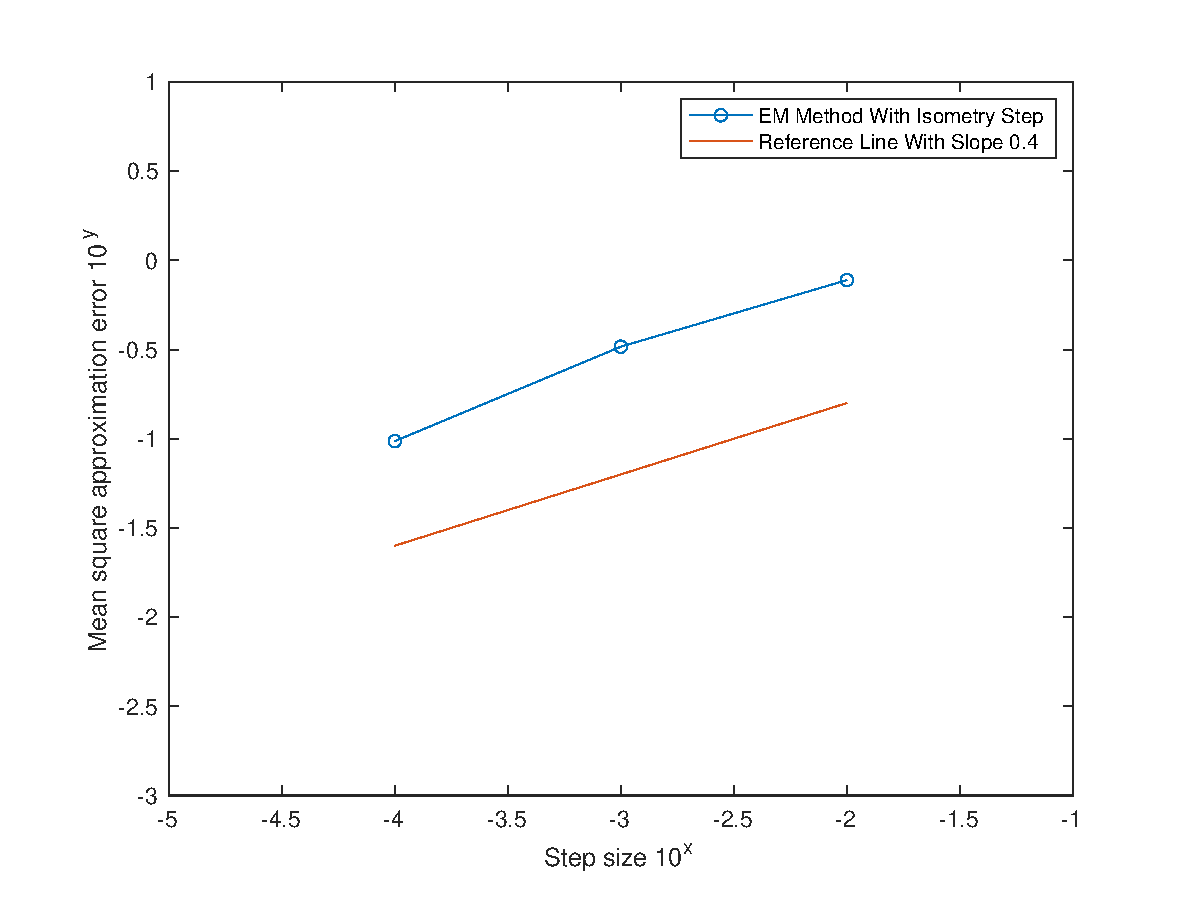
\includegraphics[width=0.45\linewidth]{isometry_EM_0.4.eps}
		\hfill
		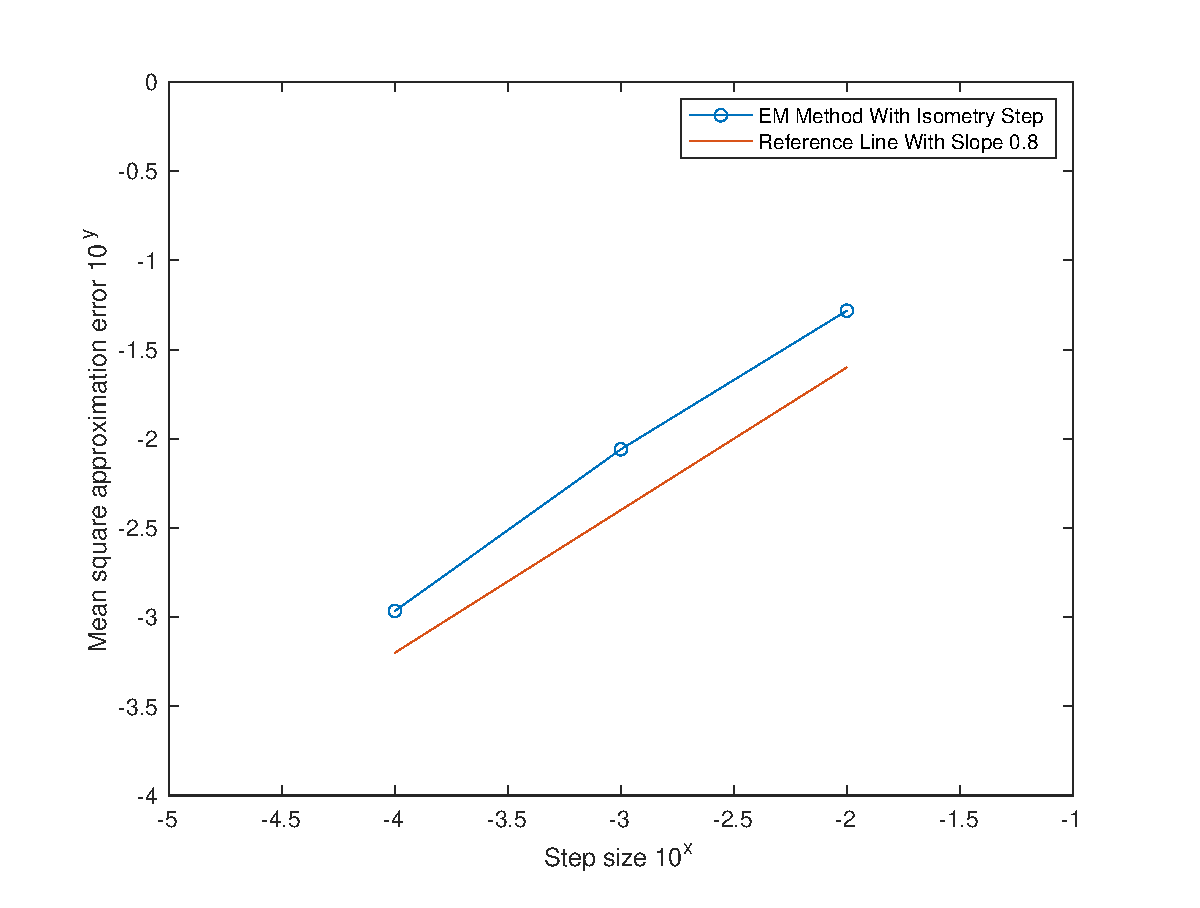
\includegraphics[width=0.45\linewidth]{isometry_EM_0.8.eps}
		\caption{在等距步长下, EM方法的$L_1$误差, 左图为$\alpha=0.4$, 右图为$\alpha=0.8$}
		\label{fig:EMsamestep}
		\vspace{-2ex}
		{}
	\end{figure}
%		
	% 定义并插入图片
	\begin{figure}[htp!]
		\centering
		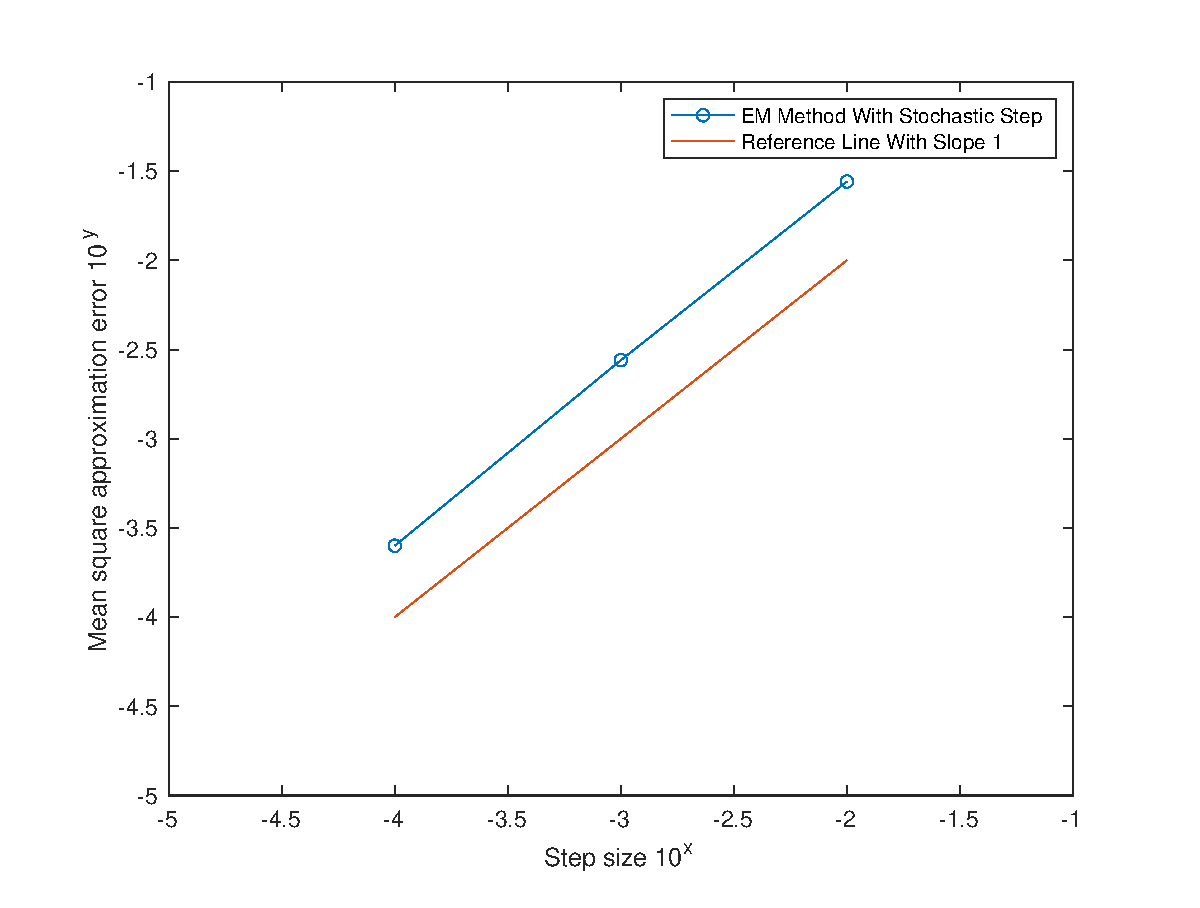
\includegraphics[width=0.45\linewidth]{stochastic_EM_0.4.eps}
		\hfill
		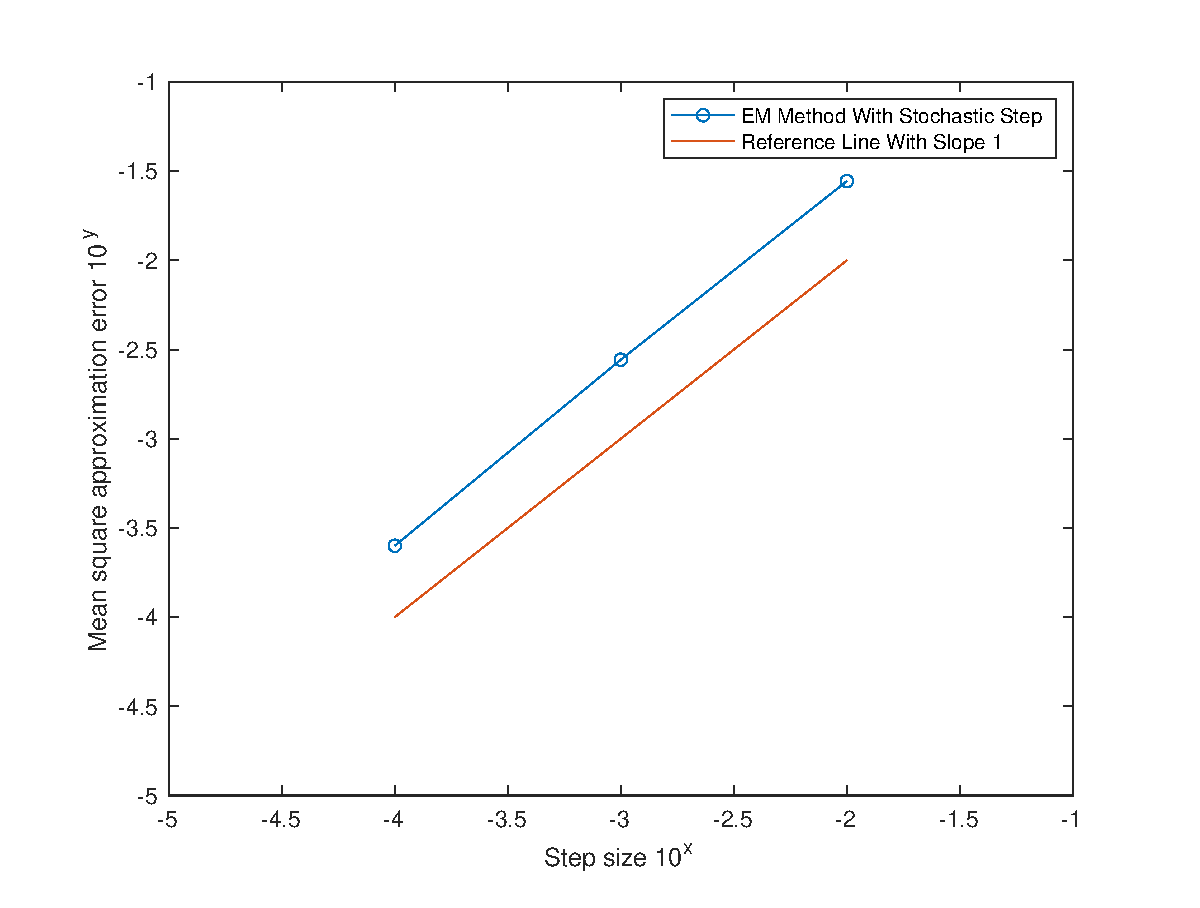
\includegraphics[width=0.45\linewidth]{stochastic_EM_0.8.eps}
		\caption{在随机步长下, EM方法的$L_1$误差, 左图为$\alpha=0.4$, 右图为$\alpha=0.8$}
		\label{fig:isometry_EM}
		\vspace{-2ex}
		{}
	\end{figure}
	
	



